%!TEX root = ../thesis.tex
本研究で開発するロボットアームは,オープンプラットフォームとしての利用のしやすさを考慮し,オフィスロボットとして最低限の機能を要求する.本章では,従来のオフィスロボットのロボットアーム調査を行い,要求仕様をまとめる.加えて,開発したロボットアームを検証する際に行う作業について,オフィスロボットが対象としている作業を基に検討する.
\section{ロボットアーム調査}
本節では,従来のオフィスロボットのロボットアーム20台を対象に調査し,以下の項目について仕様をまとめる.
\begin{itemize}
  \item アームリーチ
  \item 可搬重量
  \item 自由度
  \item エンドエフェクタ
\end{itemize}
以下では,これらの項目の詳細について述べる.

\subsection{アームリーチ}
従来のオフィスロボットのアームリーチ調査の結果(図\ref{fig:reach}参照),最小値は0.51m,最大値は0.90m,平均値および中央値はいずれも0.71mであった.この結果より,オフィス環境での作業では最低0.51m以上のアームリーチが必要であるといえるが,0.6m以下のロボットが2台であることから,対応できない作業があると想定される.また,アームリーチ0.8mを超えるロボットも10台中2台であり,このことから,0.8mを超えたアームリーチは,現在のオフィスロボットが対象としている作業には過剰であると考えられる.

以上を踏まえ,本研究ではアームリーチの要件を0.6mから0.8mの範囲に設定する.この範囲内のアームリーチであれば,基本的な作業に対応できると考えられる.
\begin{figure}[h]
  \centering
  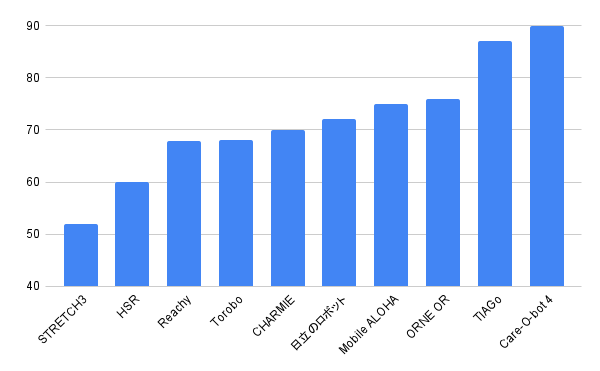
\includegraphics[width=10cm]{images/2syou/reach.png}
  \caption{Office robot arm reach survey results}
  \label{fig:reach}
\end{figure}

\subsection{可搬重量}
従来のオフィスロボットの可搬重量の最小は0.35kgであった(図\ref{fig:payload}参照).よって,現時点のオフィス作業においては0.5kg以上の可搬重量を確保できれば十分であると考えられるため,本研究では0.5kg以上を可搬重量の要件とした.
\begin{figure}
  \centering
  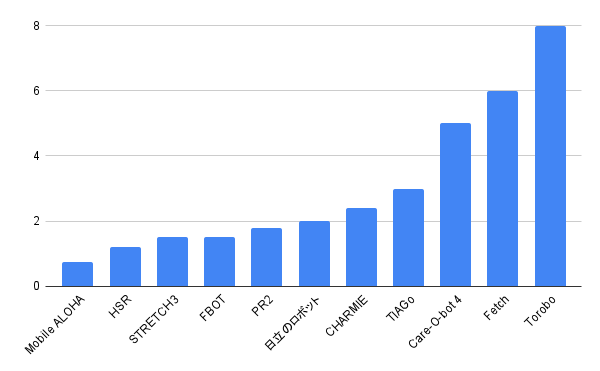
\includegraphics[width=10cm]{images/2syou/payload.png}
  \caption{Office robot payload survey results}
  \label{fig:payload}
\end{figure}
\clearpage

\subsection{自由度}
従来のオフィスロボットのアームの自由度を調査したところ,6自由度と7自由度のロボットが大半であった(\ref{fig:armDof}参照).6自由度の軸配置は,肩2軸(ピッチ,ロール),肘1軸(ロール),手首3軸(ロール,ピッチ,ヨー)で,7自由度ロボットは肩にロール軸が追加されている.7自由度アームは6自由度アームに比べて姿勢の自由度が増す一方で,アーム重量やコストが増加する.本研究ではコスト削減と軽量化を優先し,6自由度を採用した.
\begin{figure}[h]
  \centering
  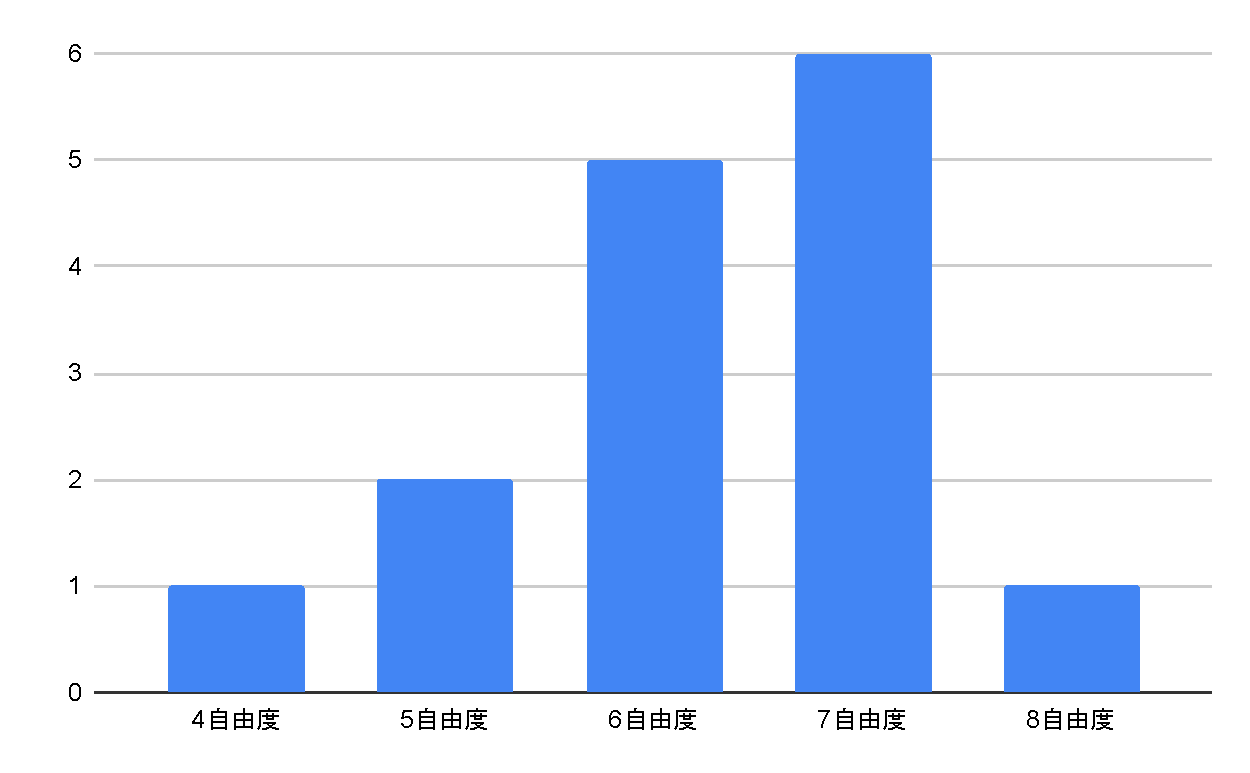
\includegraphics[width=10cm]{images/2syou/armDof.pdf}
  \caption{Office robot arm DoF survey results}
  \label{fig:armDof}
\end{figure}
\clearpage

\subsection{エンドエフェクタの形状}
従来のオフィスロボットで多く採用されているエンドエフェクタは,TIAGoのような平行グリッパ(図\ref{fig:tiago_hand}参照)である.TIAGoを開発しているPAL Robotics社が公開している動画\cite{TIAGo-movie:online}では,布,ジュース缶,スプレー缶,ジュースパック,板状物など多様な形状の物体を把持している様子が確認できる.本研究においても多様な形状の物体把持が求められるため,平行グリッパを採用した.
\begin{figure}[h]
  \centering
  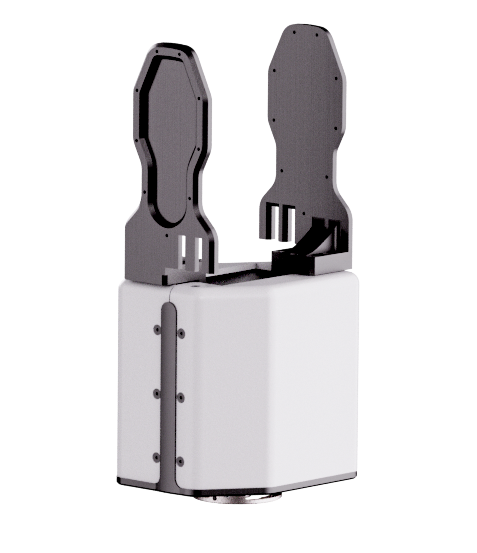
\includegraphics[width=8cm]{images/2syou/tiago_hand.png}
  \caption[End effectior of TIAGo]{End effectior of TIAGo (source: \cite{TIAGo:online})}
  \label{fig:tiago_hand}
\end{figure}
\clearpage

\subsection{オフィスロボットのロボットアームとして要求される項目}
以上を踏まえ,本研究で開発するロボットアームに,以下の項目を要求する.これを仕様として,ロボットアームのメカニズムを設計する.
\begin{itemize}
  \item 0.6m - 0.8mのアームリーチ
  \item 500g以上の可搬重量
  \item 6自由度アーム
  \item 平行グリッパのエンドエフェクタ
\end{itemize}
\newpage